\section{System Overview}
\label{sec:systemoverview}

\subsection{Use Cases}
Figure \ref{fig:pi-use-cases} shows a general overview of the use cases we have included in our prototype. A medication process can be started set off two ways:
A parent can register an alarm by using AsthmAPP. This alarm is then set of by the \code{AsthmaBuddy} instance running \footnote{The reader should take notice that the tangible user interface \ab{} differs from the program running on the \rpi{}, which is called \code{AsthmaBuddy}(note the change of font)}, giving the child a notification that it is time to take the relevant medicine.

The alternative to a registered alarm is if a child needs to take the medicine by need. In such case, the child or parent simply registers the RFID-tag before the child is guided through a quicker process (see Manuscript \ref{chp:anuscript}).  

\begin{figure}[H] 
	\centering
		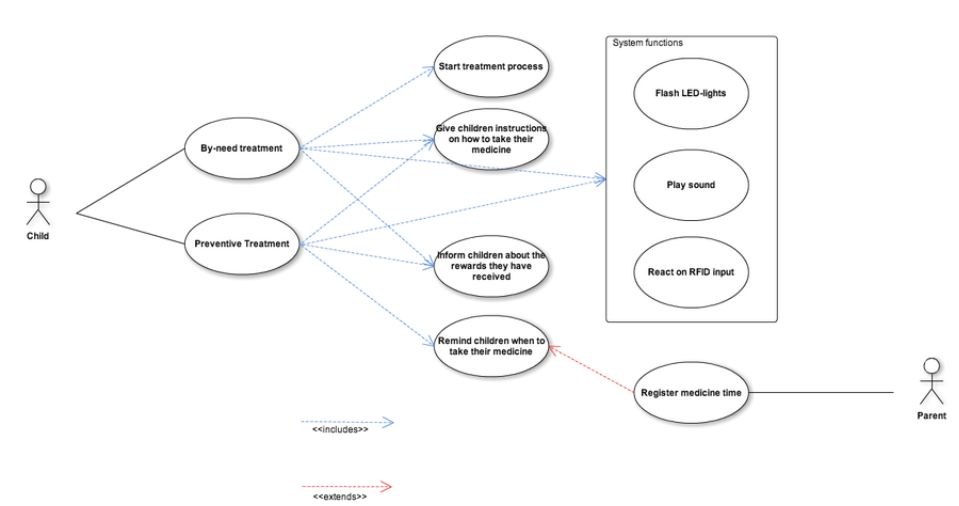
\includegraphics[width=0.8\paperwidth]{Pictures/usecases.png}
	\caption{AsthmaBuddy Use Cases}
	\label{fig:pi-use-cases}
\end{figure}

\subsection{Textual Use Cases}
\label{sec:textualusecasebyneed}

%--------- TEXTUAL USE CASE ----------
%--------- BY NEED TREATMENT ---------
\begin{table}[H]
\centering
\begin{tabular}{|p{4.0cm} | p{9.0cm} |}
\hline
\textbf{Title} & By need treatment \\
\hline
\textbf{Preconditions} & - \\
\hline 
\textbf{Scenario} & 
	\begin{enumerate}
	  \itemsep0em
	  \item User triggers treatment by holding a specific RFID-tag close to AsthmaBuddy.
	  \item System flashes LED-lights to notify user that the system is ready for use.
	  \item System plays sound to instruct the user to shake the medicine.
	  \item System plays sound to instruct user to mount the medicine on the mask and place the mask on his/her face.
	  \item User starts a treatment by interacting with AsthmaBuddy (by pressing it's hand or similar interaction).
	  \item System plays sound to count during treatment (1-2-3-4-5-6-7-8-9-10), while flashing lights for each count.
	  \item System plays sound to tell user he/she has done a good job.
	  \item System calculates reward based on health state.
	  \item System plays sound to reward user with the calculated number of stars.
	  \item System plays sound to tell the user how many stars he/she has collected totally.
	\end{enumerate}
\\
\hline
	\textbf{Extensions} & 
		x.a User aborts treatment by not continuing the sequence.
\\
\hline
\end{tabular}
\caption{Textual use case: By need treatment}
\label{tab:textual-use-case}
\end{table}


%--------- PREVENTIVE TREATMENT -------

\begin{table}[H]
\centering
\begin{tabular}{|p{4.0cm} | p{9.0cm} |}
\hline
\textbf{Title} & Planned treatment \\
\hline
\textbf{Preconditions} & The current time corresponds with the time for a planned treatment. \\
\hline 
\textbf{Scenario} & 
	\begin{enumerate}
	  \itemsep0em
	  \item The system recognizes the time for a planned treatment.
	  \item The system starts blinking with LED-lights and playing sound to notify user.
	  \item Child interacts with AsthmaBuddy, to notify that he/she is ready for the treatment.
	  \item Start instructions by playing sound, telling the user to find a grown-up that can keep watch.
	  \item System waits for interaction to make sure the user is ready.
	  \item System tells the user to mount the medicine on the mask and put the medicine towards AsthmaBuddy's face.
	  \item System plays sound to simulate breathing.
	  \item System plays sound to tell the user how easy it was to take medicines and that it is the user's turn.
	  \item System plays sound to instruct user, telling the user to shake the medicine.
	  \item System waits for interaction to make sure the user is ready.
	  \item System plays sound to instruct user to put the mask on his/her face.
	  \item System plays sound counting to 10. 
	  \item System plays sound to tell the user he/she has done a good job.
	  \item System calculates reward based on health state.
	  \item System plays sound to reward user with the calculated number of stars.
	  \item System makes a HTTPGet call to the server to find the total number of stars collected.
	  \item System plays sound to inform the user about how many stars the user has collected totally.
	\end{enumerate}
\\
\hline
	\textbf{Extensions} & 
		x.a Child does not interact with AsthmaBuddy when prompted
\\
\hline
\end{tabular}
\caption{Textual use case: By need treatment}
\label{tab:textual-use-case}
\end{table} 


\subsection{State Diagram}
\label{sec:statediagram}

In order to start the AsthmaBuddy application, we used SSH in order to gain access to the computer. We then retrieved the latest version of the source code from Git\fnurl{Git is the Source Code Management system we used}{http://git-scm.com/}, compiled it, and started running it (this process is described in Appendix \ref{app:asthmabuddy_manual}). Once AsthmaBuddy is running, it follows the state diagram depicted in Figure \ref{fig:asthmabuddy_statediagram}.  
  

\begin{figure}[H] 
	\centering
		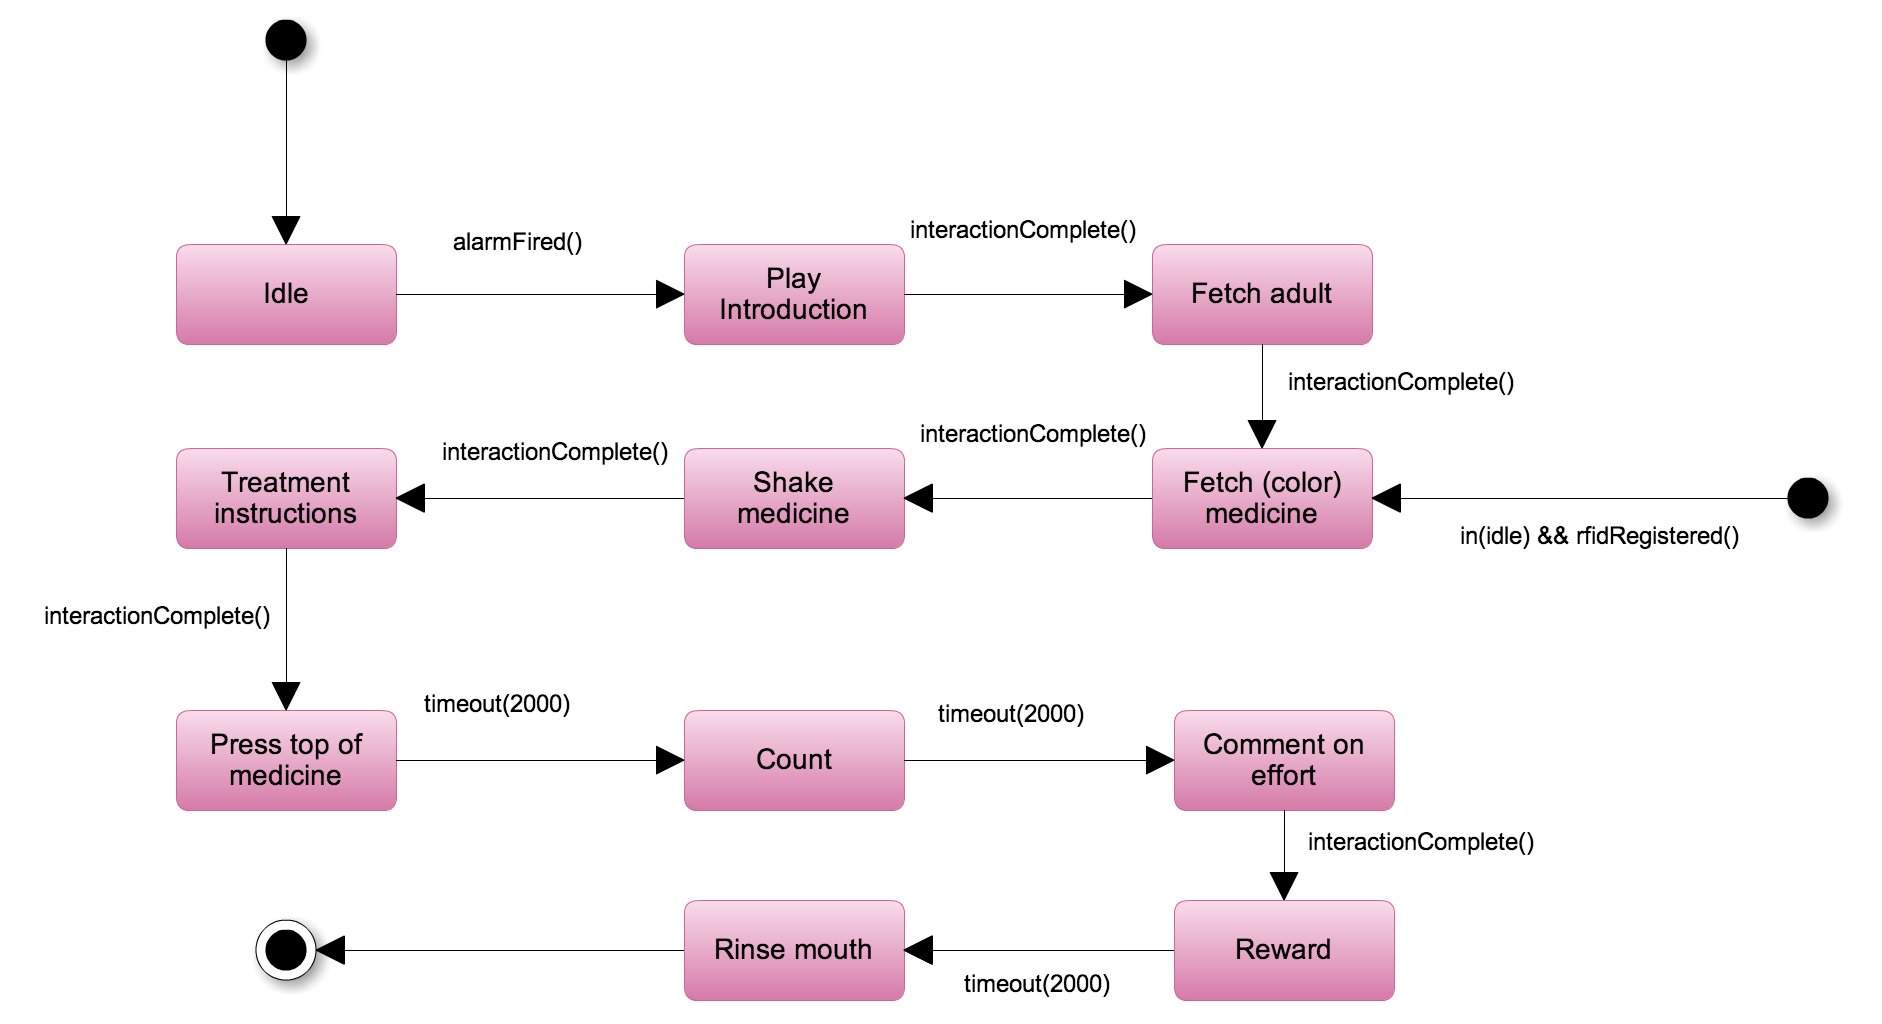
\includegraphics[width=0.7\paperwidth]{Pictures/statediagram.png}
	\caption{AsthmaBuddy State Diagram.}
	\label{fig:asthmabuddy_statediagram}
\end{figure}

\subsection{Sequence Diagram}
Figures \ref{fig:ab-sd-byneed} - \ref{fig:ab-sd-completing-treatment} shows sequence diagrams of how the system works internally. Some abstractions have been made, in order to reduce the cluster of arrows. 

\begin{sidewaysfigure}[htbp]
	\centering
		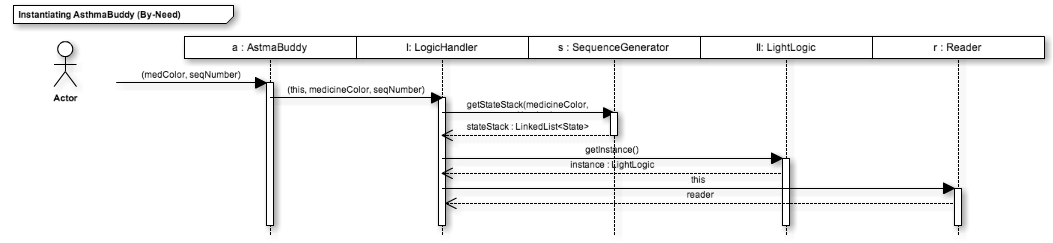
\includegraphics[scale=0.6]{Pictures/sd/sd-byneed.png}
	\caption{By Need Treatment - Sequence Diagram}
	\label{fig:ab-sd-byneed}
\end{sidewaysfigure}

\begin{sidewaysfigure}[htbp]
	\centering
		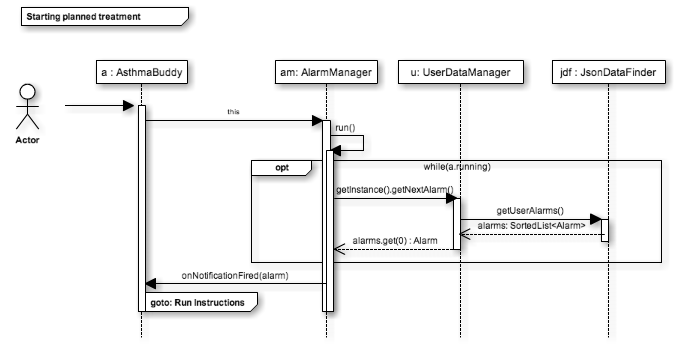
\includegraphics[scale=0.6]{Pictures/sd/sd-planned-treatment.png}
	\caption{Planned Treatment - Sequence Diagram}
	\label{fig:ab-sd-planned-treatment}
\end{sidewaysfigure}

\begin{sidewaysfigure}[htbp]
	\centering
		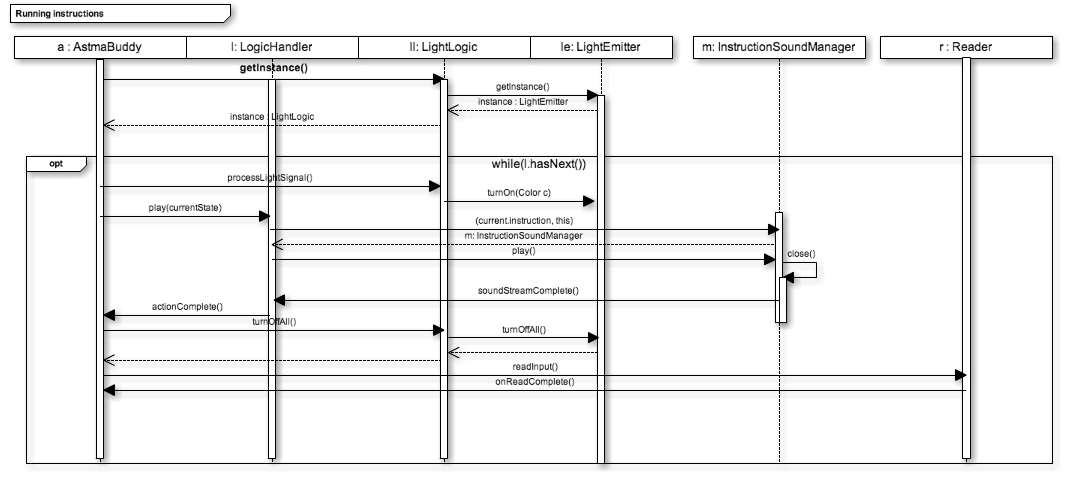
\includegraphics[scale=0.6]{Pictures/sd/sd-instructions.png}
	\caption{Playing Instructions - Sequence Diagram}
	\label{fig:ab-sd-instructions}
\end{sidewaysfigure}

\begin{sidewaysfigure}[htbp]
	\centering
		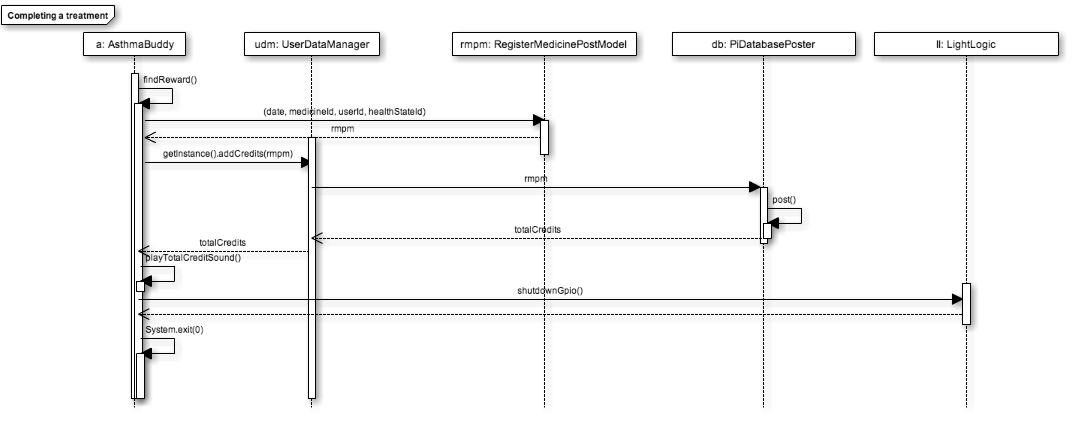
\includegraphics[scale=0.6]{Pictures/sd/sd-complete-treatment.png}
	\caption{Finishing a treatment - Sequence Diagram}
	\label{fig:ab-sd-completing-treatment}
\end{sidewaysfigure}


\begin{sidewaysfigure}[htbp]
	\centering
		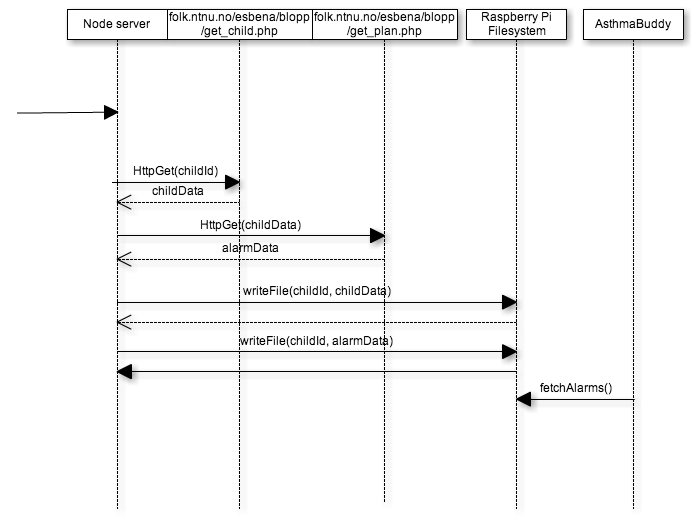
\includegraphics[scale=0.6]{Pictures/sd/sd-synchronizingv2.png}
	\caption{Synchronizing alarms - Sequence Diagram}
	\label{fig:ab-sd-synchronizing}
\end{sidewaysfigure}

\textbf{By Need Treatment}

We were not able to find a reasonable easy way to let the \buddy{} automatically be aware of the medicine that was to be taken at the start of a treatment. As a result, we used ssh into the \rpi{}, and provided the color of the medicine and the sequence number for the interaction that was to be tested.

After inserting these parameters, the \code{LogicHandler} retrieves a \code{LinkedList} of \code{Interaction}-objects that is to be played. After this sequence is ended, the system jumps to Figure \ref{fig:ab-sd-instructions}.
 
\textbf{Planned Treatment}

If an \code{AsthmaBuddy} instance is started without any parameters, it starts looking through alarm files (see Section \ref{sec:node-server}) every 60 seconds. If no alarm is returned from \code{UserDataManager}, it waits. Once an alarm is found, \code{AsthmaBuddy} is notified through \code{onNotificationFired}, which starts the treatment process. 
 
\textbf{Playing Instructions}

Playing instructions is mainly a loop of playing a sound, and turning on and off the LED-lights through the \code{LightEmitter} instance. 

\textbf{Finishing a Treatment}

When a treatment is finished, i.e. we are out of the \code{while} loop in Figure \ref{fig:ab-sd-instructions}, we register the treatment in the database. This ensures that the child is able to see the rewards in AsthmAPP. 


\subsection{Node Server}
\label{sec:node-server}
In addition to the Java application running on the \rpi{}, we developed a Node.js server\fnurl{Node.js}{http://nodejs.org/}. This backend system was developed in order to easily visualize the rewards given to a child after a treatment using \buddy{}. The initial problem is that AsthmAPP stores data to a MySQL database, with \code{childId} as the primary key for most tables. Initially, \buddy{} has no way of knowing which \code{childId} to add rewards to, or for which user alarms should be triggered. The current solution to our problem was to develop a Node.js server on AsthmaBuddy, which run as a background process. Whenever we want to switch users, AsthmAPP does an HTTP POST to this server, including the \code{childId} as a parameter. The server then retrives JSON-formatted data from our webservice, which includes the rewards a child has been given until now (for instance, by using a smartphone), and the alarms set for this user. 
When \buddy{} starts running, it checks for alarms to be set off every 60 seconds. When a child has finished a treatment, \code{AsthmaBuddy} updates the database, with the \code{childId} previously retrieved, and the number of stars a child collected during his/her treatment. With the data retrieved from the database, \buddy{} has the capability to tell the user how many stars a child has collected\footnote{Since this is a prototype, this functionality only works until a child has collected 20 stars. It became cumbersome to handle rewards totalling more than 20 stars}. This process is shown in Figure \ref{fig:ab-sd-synchronizing}.

